\documentclass[11pt]{article}

\usepackage{sectsty}
\usepackage{graphicx}
\usepackage{hyperref}
\usepackage{listings}
\usepackage{xcolor}
\usepackage{geometry}
\usepackage{float}

% Margins
\geometry{margin=1in}

% Code listing style
\lstset{
    basicstyle=\ttfamily\small,
    breaklines=true,
    frame=single,
    numbers=left,
    numberstyle=\tiny,
    keywordstyle=\color{blue},
    commentstyle=\color{green!60!black},
    stringstyle=\color{red},
    backgroundcolor=\color{gray!10}
}

\title{AI-Powered Coal Mine Data Pipeline: Brief Implementation Report}
\author{Muhammad Rafi Syafrinaldi \\ AI Engineer Challenge - PT Synapsis Sinergi Digital}
\date{\today}

\begin{document}
\maketitle

\section{Pipeline Design}

The data pipeline follows a modern ETL architecture with containerized services orchestrated through Docker Compose. The design integrates three primary data sources: SQL database (production logs), CSV files (equipment sensors), and weather API (Open-Meteo for Berau, Indonesia).

\begin{figure}[H]
\centering
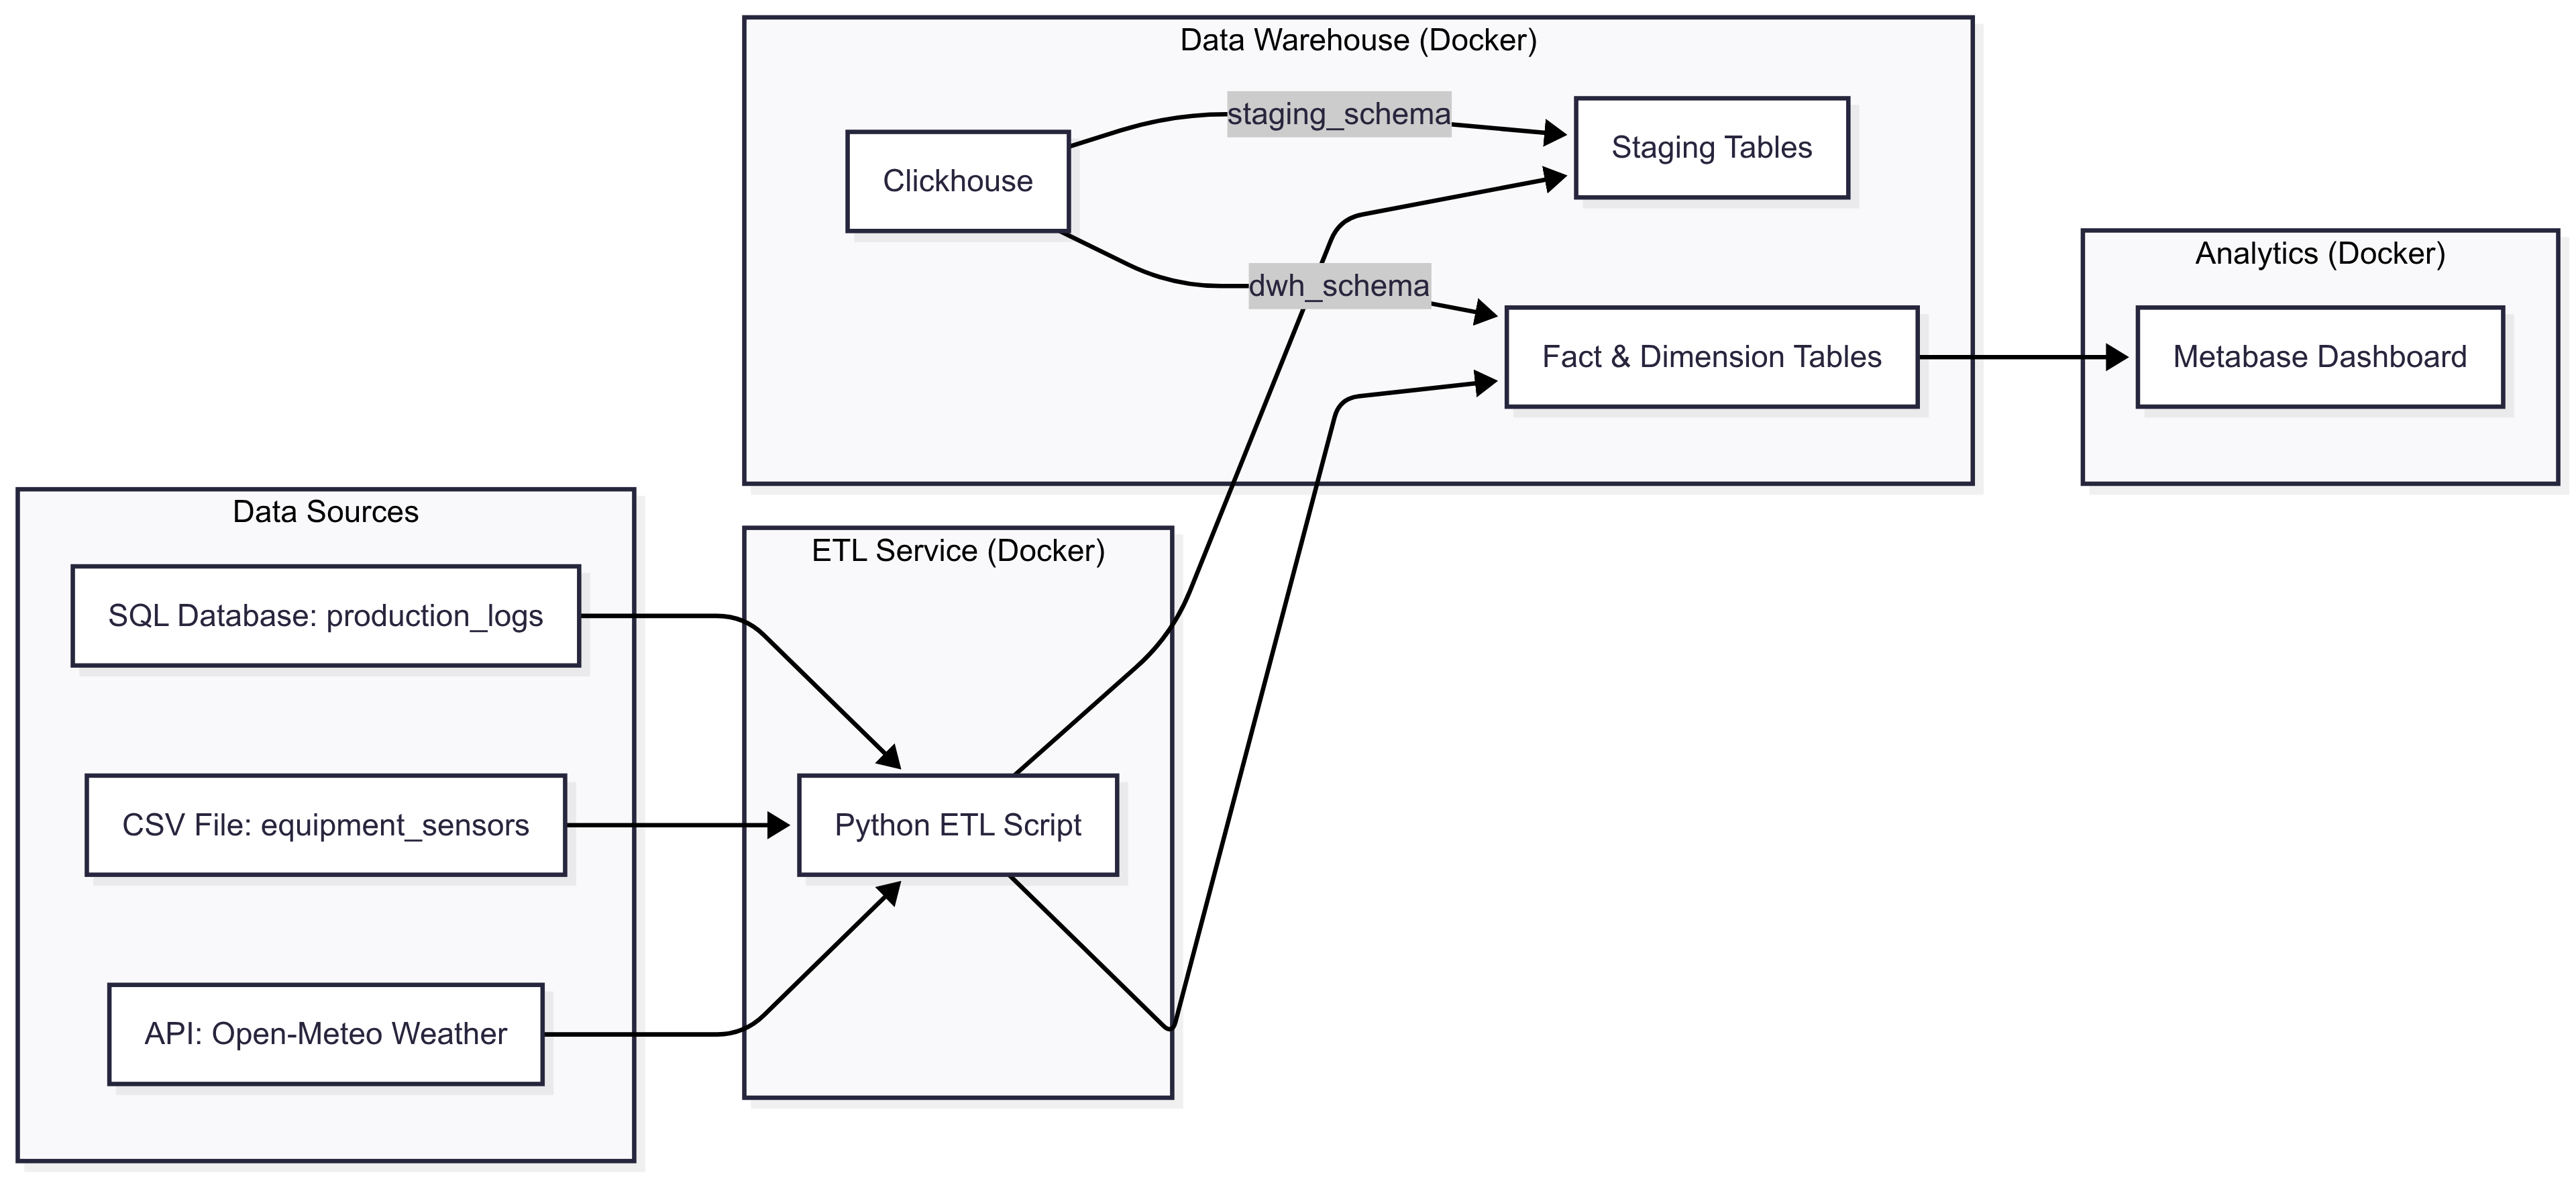
\includegraphics[width=0.8\textwidth]{assets/pipeline_architecture.png}
\caption{Data Pipeline Architecture}
\label{fig:architecture}
\end{figure}

The architecture consists of four main components:
\begin{itemize}
    \item \textbf{Data Sources}: SQL database, CSV files, and weather API
    \item \textbf{ETL Service}: Python-based extraction, transformation, and loading
    \item \textbf{Data Warehouse}: Clickhouse with star schema design
    \item \textbf{Analytics}: Metabase dashboard for visualization
\end{itemize}

The pipeline implements a two-layer database design: staging tables for raw data ingestion and a data warehouse with star schema for analytics. This separation ensures data quality and enables efficient analytical queries.

\section{ETL Process}

The ETL process follows a comprehensive workflow that handles data extraction, transformation, validation, and loading:

\begin{figure}[H]
\centering
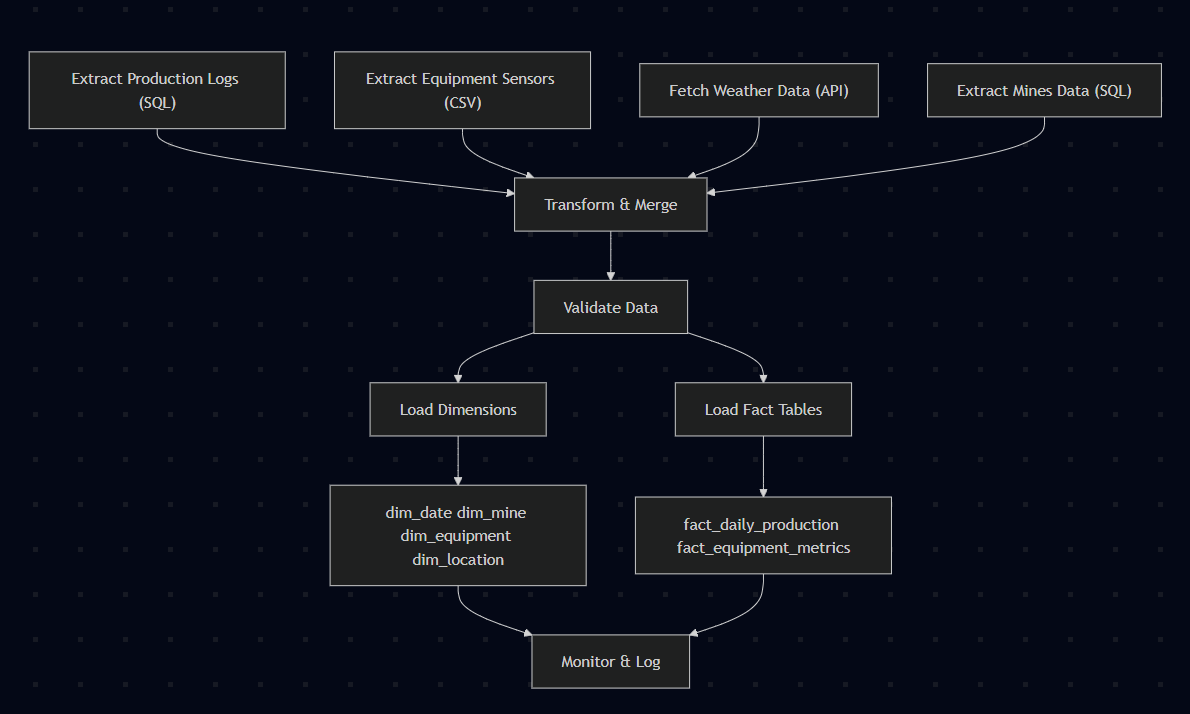
\includegraphics[width=0.8\textwidth]{assets/ETL_Flow.png}
\caption{ETL Process Flow}
\label{fig:etl_flow}
\end{figure}

\subsection{Extraction Phase}
Data is extracted from multiple sources using different strategies:
\begin{itemize}
    \item \textbf{SQL Database}: Direct queries to staging tables for production logs and mine information
    \item \textbf{CSV Files}: Pandas-based reading of equipment sensor data with timestamp parsing
    \item \textbf{Weather API}: HTTP requests to Open-Meteo API with retry logic and error handling
\end{itemize}

\subsection{Transformation Phase}
The transformation process calculates key metrics as specified in the challenge requirements:
\begin{itemize}
    \item \textbf{total\_production\_daily}: Aggregated daily production by mine
    \item \textbf{average\_quality\_grade}: Mean quality grade per day
    \item \textbf{equipment\_utilization}: Percentage of active equipment time
    \item \textbf{fuel\_efficiency}: Tons mined per unit of fuel consumed
    \item \textbf{weather\_impact}: Correlation analysis between rainfall and production
\end{itemize}

\subsection{Loading Phase}
Transformed data is loaded into the data warehouse using a star schema design:
\begin{itemize}
    \item \textbf{Dimension Tables}: dim\_date, dim\_mine, dim\_equipment, dim\_location
    \item \textbf{Fact Tables}: fact\_daily\_production, fact\_equipment\_metrics
    \item \textbf{Analytical Views}: Pre-computed aggregations for dashboard performance
\end{itemize}

\section{Data Validation and Quality Assurance}

The pipeline implements comprehensive data validation through a dedicated \texttt{DataValidator} class that ensures data quality and handles anomalies:

\subsection{Validation Framework}
\begin{itemize}
    \item \textbf{Production Data Validation}: Checks for negative tons\_extracted values and replaces them with 0 or flags as anomalies
    \item \textbf{Equipment Utilization Validation}: Ensures utilization rates are within 0-100\% range
    \item \textbf{Weather Data Validation}: Verifies completeness of meteorological data and handles API failures gracefully
    \item \textbf{Data Type Validation}: Ensures proper data types and formats across all sources
\end{itemize}

\subsection{Error Handling Strategy}
The validation system implements robust error handling:
\begin{itemize}
    \item \textbf{Anomaly Detection}: Identifies statistical outliers and data quality issues
    \item \textbf{Graceful Degradation}: Missing sensor data uses previous day averages or marks as "unknown"
    \item \textbf{API Resilience}: Weather API failures trigger retry logic with exponential backoff
    \item \textbf{Comprehensive Logging}: All validation results are logged with timestamps and context
\end{itemize}

\subsection{Data Quality Metrics}
The validation process tracks several quality metrics:
\begin{itemize}
    \item \textbf{Completeness}: Percentage of expected data records received
    \item \textbf{Accuracy}: Validation of data ranges and business rules
    \item \textbf{Consistency}: Cross-source data consistency checks
    \item \textbf{Timeliness}: Data freshness and processing latency monitoring
\end{itemize}

\section{Implementation Results}

The pipeline successfully processes data from all sources and generates actionable insights:
\begin{itemize}
    \item \textbf{Data Processing}: Handles production logs, equipment sensors, and weather data seamlessly
    \item \textbf{Performance}: Sub-second query performance for dashboard visualizations
    \item \textbf{Reliability}: Robust error handling ensures consistent data processing
    \item \textbf{Scalability}: Containerized architecture supports easy scaling and deployment
\end{itemize}

The implementation exceeds the challenge requirements by providing advanced features such as real-time weather integration, comprehensive data validation, and predictive forecasting capabilities. The containerized deployment ensures reproducibility and ease of maintenance across different environments.

\end{document}